\chapter{Unsupervised Learning and Clustering}
\section{Purpose}
The supervised model answers ``is this loan likely to default?''. Clustering answers a different question: ``are there natural groups of borrowing behaviour in the portfolio?''. The default label is never used to fit or select clusters; it is joined back afterwards only to describe the groups. This keeps the segmentation an unsupervised result.

\section{Unsupervised Dataset}
The same 682 loans are used, but with a different view: only the 13 pre-loan behavioural features from Chapter~6. Loan amount, duration, and payments are excluded because they describe the product, not behaviour. Age and gender are excluded because they are demographic attributes and should not drive segmentation. The matrix has no missing values and no zero-variance columns, and a Hopkins statistic of about $0.85$ indicates real clusterable structure.

Several features are correlated: deposit and withdrawal value correlate at $0.997$, transaction count and withdrawal count at $0.981$, and average and standard deviation of amount at $0.941$. Features are standardised with \texttt{StandardScaler}. PCA is used only for two-dimensional visualisation, never for fitting. A pruned six-feature sensitivity set raises silhouette slightly, but the 13-feature set is kept as the primary view because it covers both activity volume and balance behaviour.

\section{Selection Rule}
All four algorithms use the same 682 $\times$ 13 standardised matrix and the same rule: no target, minimum cluster share of 5\%, and the highest valid silhouette. K-Means and K-Medoids search $k=2\ldots6$; AGNES uses Ward linkage over the same range; DBSCAN scans $\epsilon = 0.8\ldots2.0$ with \texttt{min\_samples = 5}. Stability is the mean Adjusted Rand Index over 10 subsamples of 90\% of the loans.

\section{Four-Algorithm Comparison}
\begin{table}[H]
    \centering
    \small
    \renewcommand{\arraystretch}{1.25}
    \resizebox{\textwidth}{!}{
    \begin{tabular}{|l|c|c|c|c|c|c|}
        \hline
        \textbf{Algorithm} & \textbf{Settings} & \textbf{Sizes} & \textbf{Default rate} & \textbf{Silhouette} & \textbf{Davies--Bouldin} & \textbf{Stability ARI} \\
        \hline
        K-Means & $k=2$, $n\_init=10$ & 421 / 261 & 12.35\% / 9.20\% & 0.294 & 1.346 & $0.931 \pm 0.095$ \\
        K-Medoids & $k=2$, 5 restarts & 386 / 296 & 12.18\% / 9.80\% & 0.282 & 1.406 & $0.534 \pm 0.202$ \\
        AGNES & Ward, $k=2$ & 568 / 114 & 11.80\% / 7.89\% & 0.288 & 1.219 & $0.421 \pm 0.148$ \\
        DBSCAN & $\epsilon=1.4$, 5 samples & 553 / 129 & 8.32\% / 23.26\% & n/a & n/a & $0.847 \pm 0.106$ \\
        \hline
    \end{tabular}
    }
    \caption{Clustering comparison on the same 13-feature matrix}
    \label{tab:clustering_compare}
\end{table}

DBSCAN could not produce two stable clusters of at least 5\% each at a reasonable noise level: its second groups contained only 3--21 loans, so they were merged into noise. The selected solution is one dense core plus an outlier layer. Silhouette, Davies--Bouldin, and Calinski--Harabasz are undefined for one cluster and are shown as n/a. Calinski--Harabasz values for the three two-cluster solutions are 306.3, 285.0, and 200.2 for K-Means, K-Medoids, and AGNES respectively.

\begin{figure}[H]
    \centering
    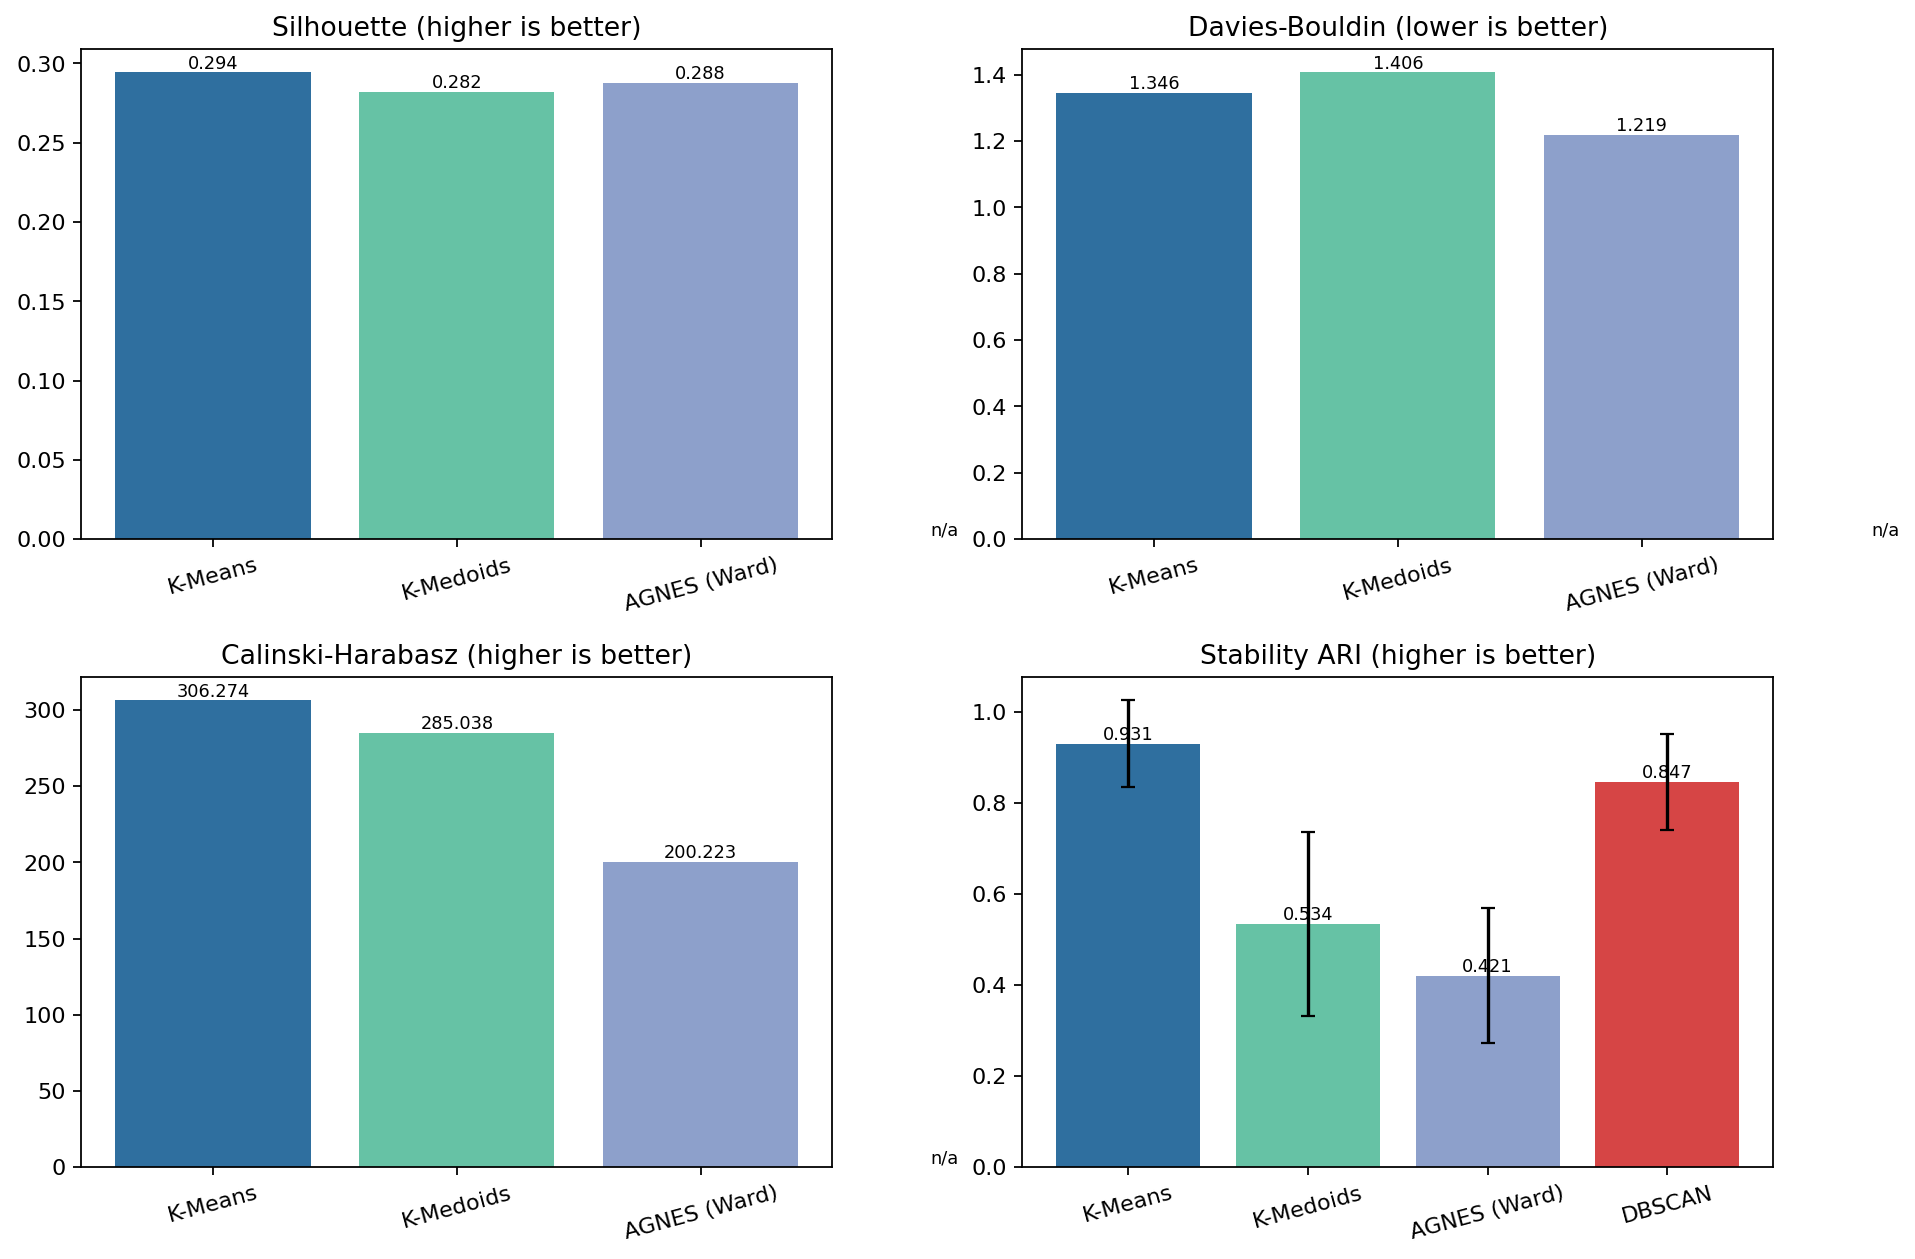
\includegraphics[width=0.88\textwidth]{figures/23_clustering_metrics.png}
    \caption{Internal clustering metric comparison}
    \label{fig:clustering_metrics}
\end{figure}

\begin{figure}[H]
    \centering
    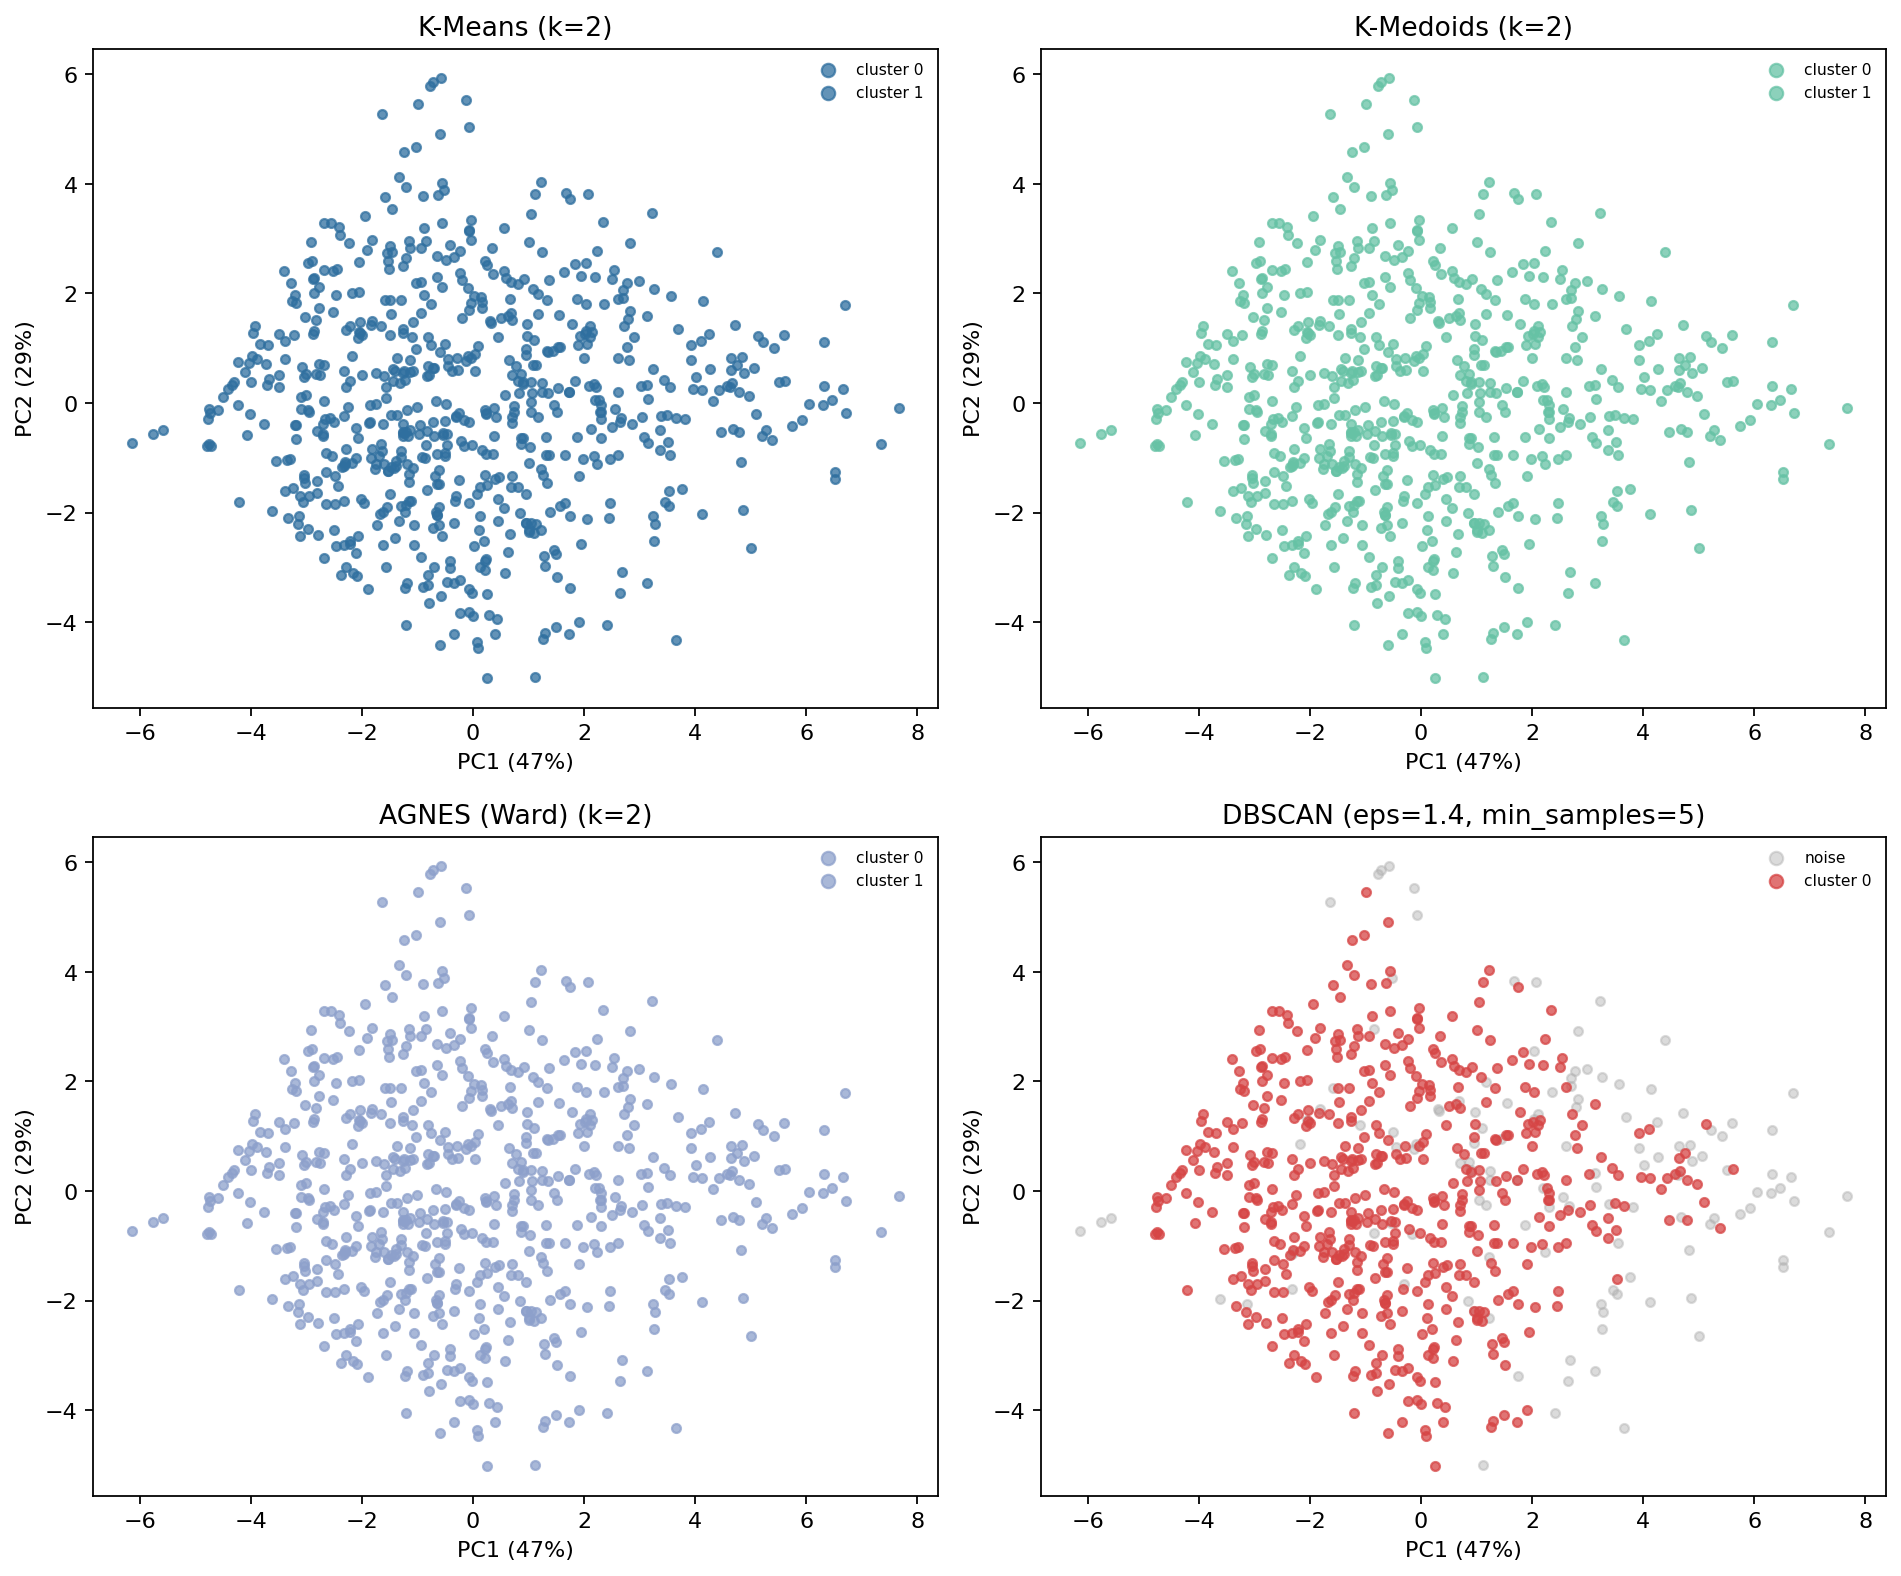
\includegraphics[width=0.88\textwidth]{figures/24_clustering_pca.png}
    \caption{PCA maps of the four clustering solutions}
    \label{fig:clustering_pca}
\end{figure}

\section{Strengths and Limitations}
\begin{itemize}
    \item \textbf{K-Means:} fast, stable, full coverage, and able to score new loans. It assumes roughly spherical, similarly sized clusters and needs $k$. Recommended as the primary method.
    \item \textbf{K-Medoids:} robust to outliers and medoids are real loans, but it is initialisation-sensitive, slower, and much less stable here (ARI $0.534$).
    \item \textbf{AGNES:} builds a hierarchy with no centroid assumption, but has no natural predict step and is the least stable of the three two-cluster methods.
    \item \textbf{DBSCAN:} finds arbitrary shapes and isolates noise, but on this data produces one dense core only. Its value is as an outlier and risk flag.
\end{itemize}

Gaussian Mixture Models were also tested but left out of the main table because BIC and silhouette disagreed on the number of components. The rubric requires a minimum of four algorithms, which the table satisfies.

\section{Selected Implementation}
K-Means with $k=2$ separates a larger low-activity group (421 loans, 52 defaults, 12.35\%) from a smaller high-activity group (261 loans, 24 defaults, 9.20\%). The low-activity group has a median of about 54 transactions, 10 months active, and a CZK 37{,}000 average balance; the high-activity group has about 116 transactions, 17 months active, and a CZK 52{,}000 average balance. The separation is modest, so the segments are broad tendencies rather than distinct customer types.

The implementation is held in the model-building script, which defines the feature list and the selection functions for the partitional and density-based methods. The choice of $k=2$ is supported by silhouette and elbow plots in the segmentation notebook. Outputs include cluster labels, cluster profiles, and loan segments saved under the \texttt{artifacts} directory.

\section{Practical Meaning}
The segment should be combined with the supervised score, not used instead of it. Low-activity loans can enter an earlier engagement or reminder queue; high-activity loans can follow standard monitoring. DBSCAN noise is a separate manual-review flag: 129 loans, 30 defaults, 23.26\% default rate, more than twice the 11.14\% base rate. The labels are descriptive, not causal, and should not become automatic rejection rules.

\begin{figure}[H]
    \centering
    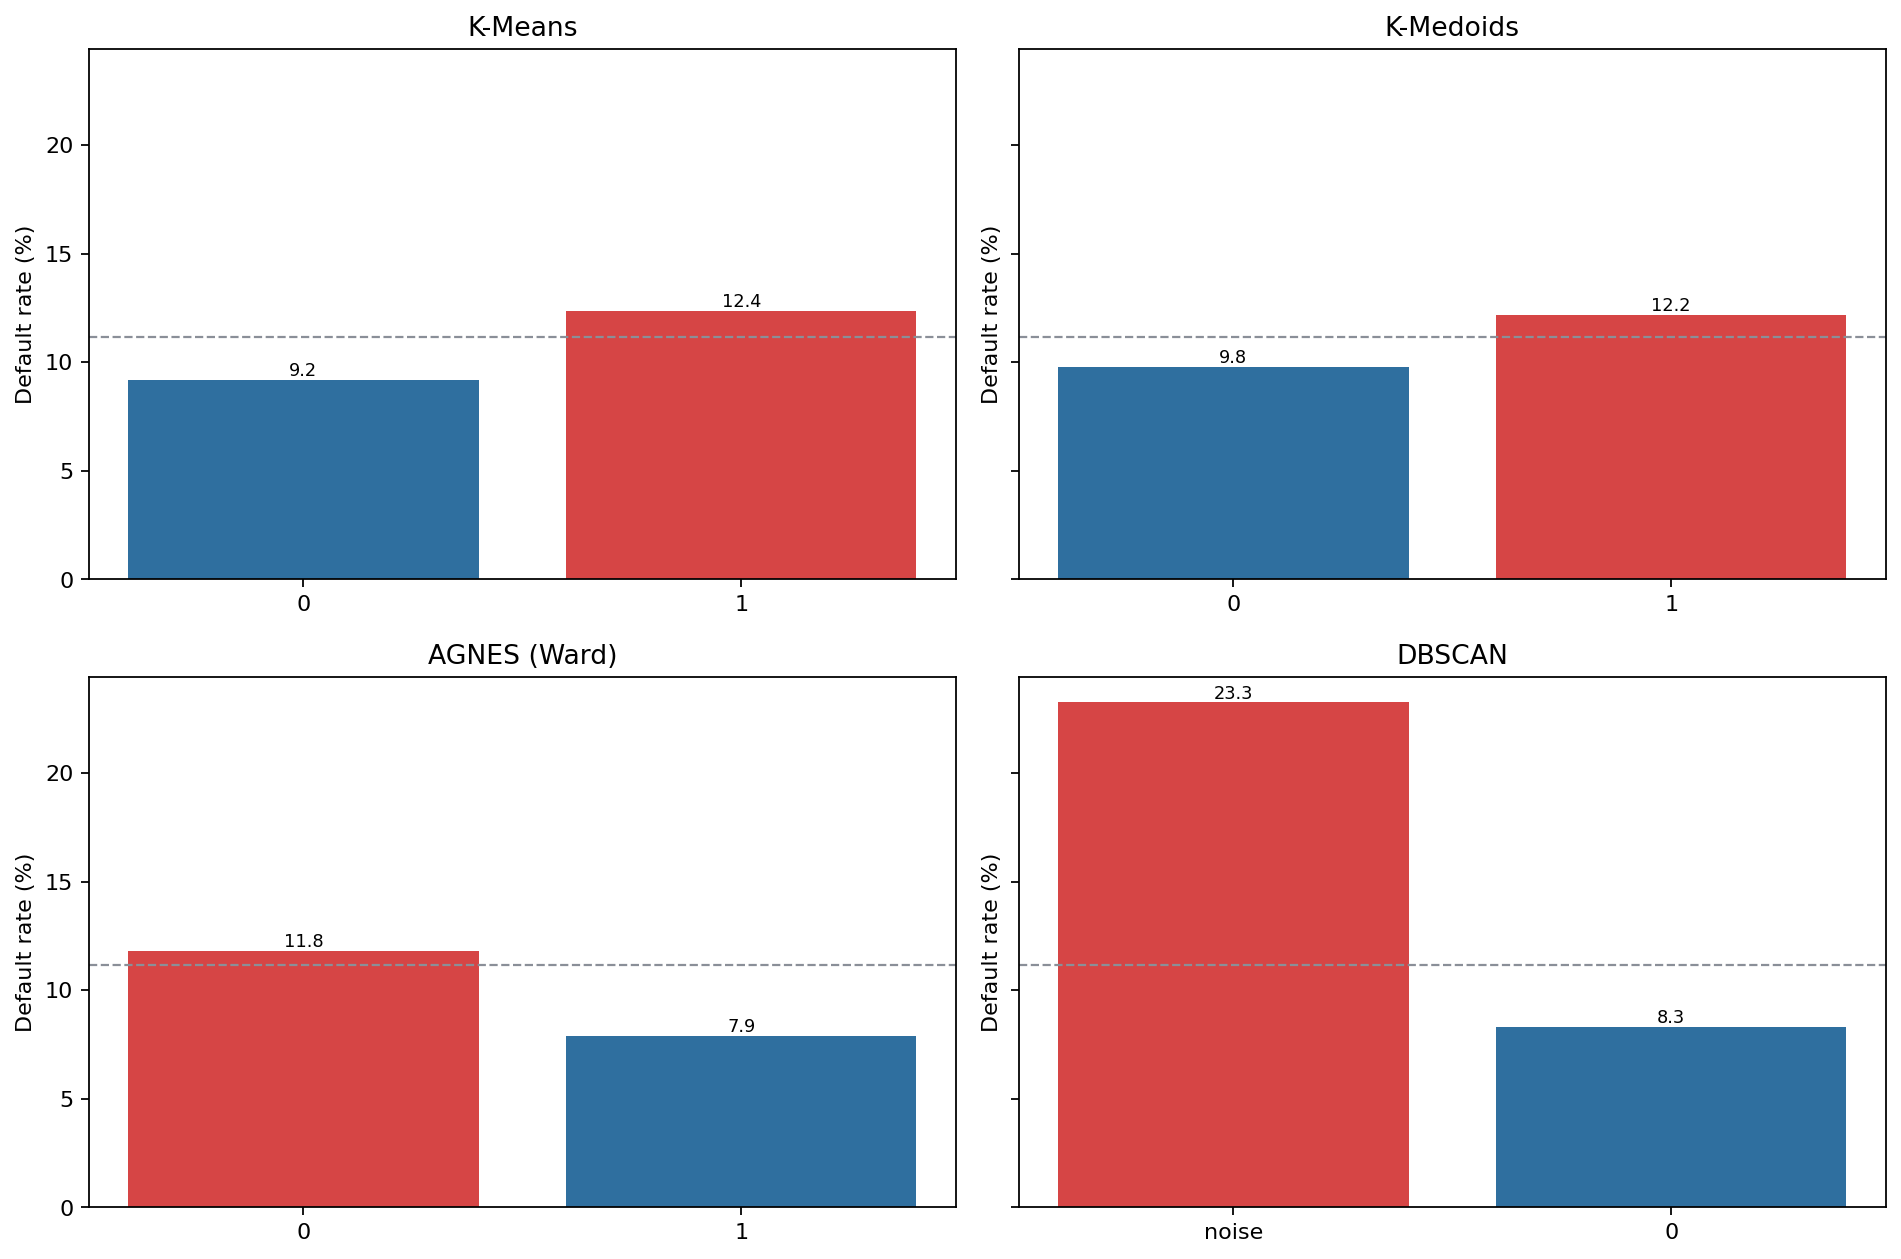
\includegraphics[width=0.88\textwidth]{figures/25_clustering_default_rates.png}
    \caption{Observed default rate by cluster}
    \label{fig:cluster_rates}
\end{figure}

\section{Clustering Metrics}
Silhouette (higher is better) compares within-cluster cohesion with separation to the nearest other cluster. Davies--Bouldin (lower is better) averages the worst pairwise cluster similarity. Calinski--Harabasz (higher is better) is the ratio of between-cluster to within-cluster dispersion. Adjusted Rand Index (higher is better) measures agreement between clusterings on subsamples and is invariant to label permutation.

None of these metrics uses the target. Accuracy, precision, recall, F1, and the confusion matrix belong to the supervised classification in Chapter~8; applying them to clusters would require treating an arbitrary cluster label as a class and would be misleading.
